\item \points{3} \points{3w} {\bf Train and Analysis}

Once you have completed problems 1 and 2, you can train your few shot classification model. You should observe both the support and query losses go down, and the query accuracy go up. Now we will examine how the performance varies for different size problems.
Train models for the following values of $K$ and $N$:
\begin{itemize}
    \item $K = 1$, $N=2$ %, you should be able to achieve about 90\% accuracy.
    \item $K = 2$, $N=2$ %, you should be able to achieve about 80\% accuracy.
    \item $K = 1$, $N=3$ %, you should be able to achieve about 75-80\% accuracy.
    \item $K = 1$, $N=4$ %, you should be able to achieve about 70\% accuracy.
\end{itemize}
% $K: [1, 5, 10]$
% $N: [5, 20, 50]$

Example code:
\begin{verbatim}
    python main.py --num_shot K --num_classes N
\end{verbatim}  

For checking training results and/or taking a screenshot for the writeup, use:
\begin{verbatim}
    tensorboard --logdir runs/
\end{verbatim}

You should start with the case $K=1 , N=2$ as it can aid you in the implementation and debugging process. Your model should be able to achieve a query set accuracy of above 90\% in this first two scenarios scenario on held-out test tasks, around 80\% in the third scenario, and around 70\% in the final scenario.

\begin{figure}
    \centering
    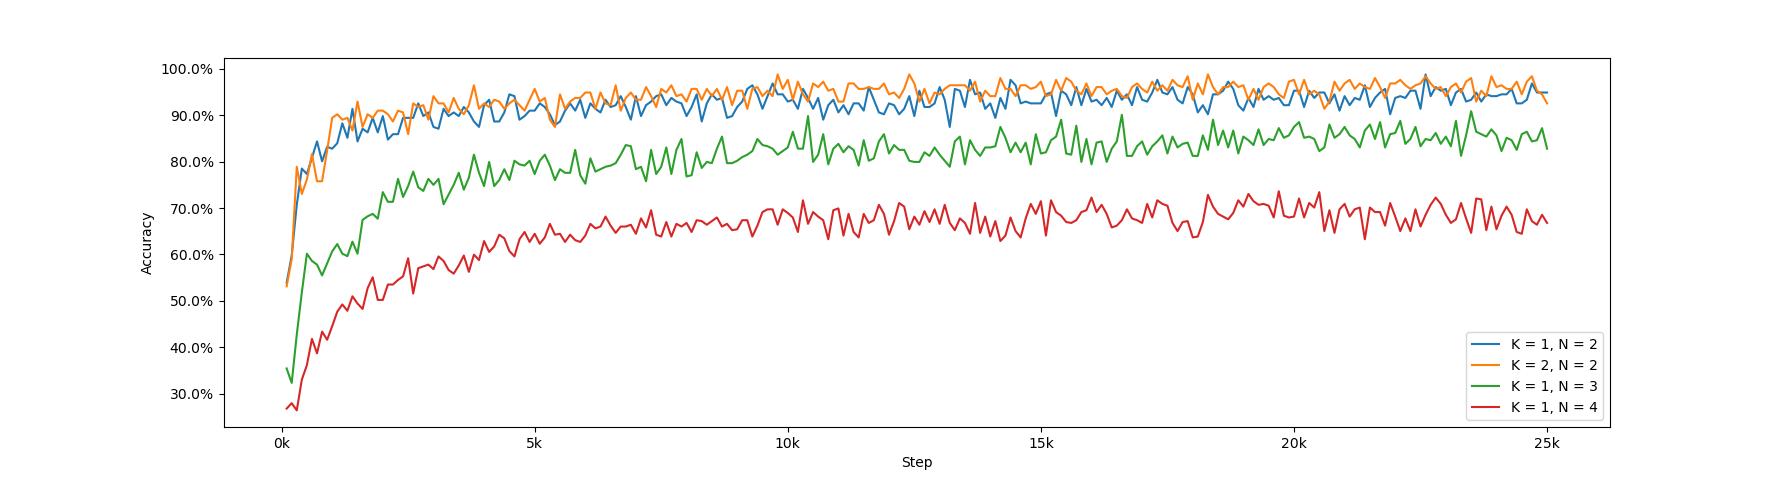
\includegraphics[width=\linewidth]{./figures/accuracy.png}
    \vspace{-5mm}
    \caption{Tensorboard plot of the meta-test query set classification accuracy over training iterations for all configurations.}
    \label{accuracy}
\end{figure}

    We have provided in Figure \ref{accuracy} a unified view of the meta-test query set classification accuracy over training iterations for all above mentioned configurations. Answer the following questions:

\begin{enumerate}
    \item How does increasing the number of classes affect learning and performance?
    \item How does increasing the number of examples in the support set affect performance?    
\end{enumerate}

\clearpage